\chapter{Race Condition}

\section{Introduzione}

Una “concorrenza incontrollata” può portare a un comportamento non deterministico
(cioè un programma può mostrare un comportamento diverso per lo stesso insieme
di input).
Una \textit{race condition} si verifica in qualsiasi scenario in cui due (o più)
thread possono
produrre un comportamento diverso, a seconda del thread che viene eseguito per primo.
Le race conditions possono derivare da flussi di controllo affidabili o non
affidabili.\\
I \textit{flussi di controllo affidabili} (\textbf{trusted}) sono thread
strettamente correlati tra di loro che fanno parte dello stesso programma.
Invece, un \textit{flusso di controllo non affidabile} (\textbf{untrusted})
è un'applicazione o un processo separato, spesso di origine sconosciuta,
che viene eseguito in contemporanea.\\

Tre proprietà sono necessarie perché una race conditions esista:
\begin{enumerate}
    \item \textit{Concurrency property}: Almeno due flussi di controllo
          devono essere eseguiti simultaneamente.
    \item \textit{Shared object property}: Deve esistere almeno un oggetto
          condiviso ed
          essere accessibile da
          entrambi i flussi concorrenti.
    \item \textit{Change state property} (Cambiare la proprietà di stato):
          Almeno uno dei flussi di
          controllo deve modificare lo stato dell'oggetto in condivisione.
\end{enumerate}

\section{Race Window}

Le Race Condition sono un difetto del software e sono una frequente fonte di
vulnerabilità.
Sono particolarmente insidiose perché dipendono dal timing e si manifestano
sporadicamente. Di conseguenza, sono difficili da rilevare, riprodurre ed
eliminare e possono
causare errori come la corruzione dei dati o crash.
Esse si manifestano in vari ambienti di runtime, compresi i sistemi operativi
che devono
controllare l'accesso alle risorse condivise, soprattutto attraverso la
programmazione dei vari
processi. Ci può essere concorrenza anche in presenza di un unico processore.
Da notare che è responsabilità del programmatore assicurarsi che il suo codice
sia correttamente
sequenziato, indipendentemente da come gli ambienti di runtime programmano
l'esecuzione
della programmazione.
La loro eliminazione inizia con l'identificazione delle \textit{Race Window}.
Una race window è un
segmento di codice che accede all'oggetto condiviso in modo da aprire una
finestra di opportunità
durante la quale altri flussi concorrenti potrebbero "correre dentro" (race in)
e alterare
l'oggetto. Fondamentalmente è una zona di codice sottoposta a più flussi di
controllo.
Una race window non è protetta da un lock o da qualsiasi altro meccanismo.
Se viene
protetta da una lock o simili viene detta “\textit{sezione critica}”.

\paragraph{Esempio.}\ \\

Gli esempi più subdoli possono dipendere anche da come è fatto il processore !
Prendiamo in considerazione il seguente codice:

\begin{figure}[H]
    \centering
    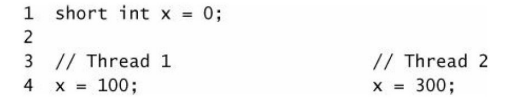
\includegraphics[width=10cm, keepaspectratio]{capitoli/secure_coding/img/cap_6/esempio1.png}
    \caption{Codice di due thread.}
\end{figure}

Come possiamo notare, i due thread assegnano un valore diverso alla stessa variabile
condivisa. Queste istruzioni
possono essere eseguite in modo diverso a livello architetturale.

\begin{figure}[H]
    \centering
    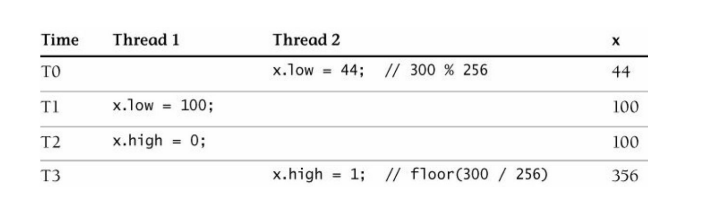
\includegraphics[width=10cm, keepaspectratio]{capitoli/secure_coding/img/cap_6/esempio1_tab.png}
    \caption{Tabella che descrive l'ordine di esecuzione delle istruzioni.}
\end{figure}

La race windows in questo caso, sono gli assegnamenti da entrambe le parti.
I registri possono essere
trattati come due metà differenti, indipendentemente dalla dimensione.
Come il compilatore
compila e come il processore si organizza è trasparente al programmatore.
Supponiamo che l'assegnamento venga effettuato in due parti da 8 bit.
Il thread 2 scrive 300, cioè $255+45$. Prima setta la parte bassa,
cioè la parte meno
significativa, a $45$; quella più significativa ad $255$.
$300$ infatti non ci sta in 8 bit.
Nel mentre però arriva il thread 1 che setta solo la parte bassa, quella meno \
significativa a $100$.
Alla fine la variabile \verb|x| conterrà il valore $100+255=355$.

\section{Race Condition su File}

Anche file e directory sono oggetti condivisi.
Le sequenze di accesso ai file in cui un file viene aperto, letto o scritto,
chiuso ed
eventualmente riaperto da funzioni separate chiamate in un certo intervallo di
tempo sono
regioni fertili per le race conditions. I file aperti sono condivisi da
peer threads, e i file system
possono essere manipolati da processi indipendenti.

\paragraph{Esempio.}\ \\

\begin{wrapfigure}{l}{0.5\textwidth}
    \centering
    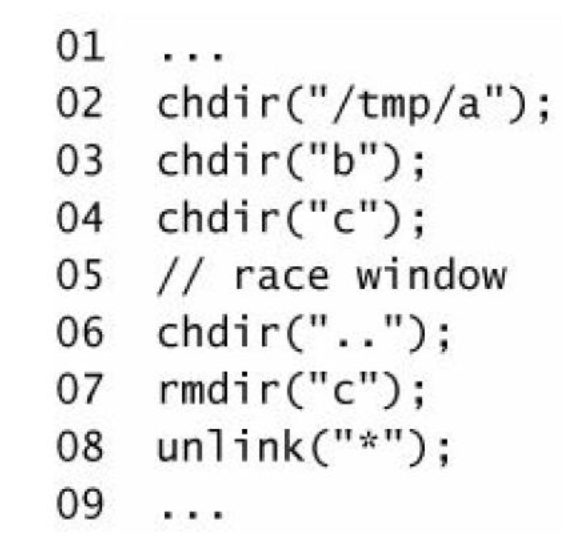
\includegraphics[width=0.4\textwidth, keepaspectratio]{capitoli/secure_coding/img/cap_6/esempio_dir.png}
\end{wrapfigure}

In questo codice avviene un cambio forzato di directory.
Con le linee 2, 3, 4 ci spostiamo in
\verb|/tmp/a/b/c|.
C'è una race window tra le linee 4 e 6. La linea 6 consiste
praticamente nell'andare in \verb|/tmp/a/b| e con la 7 si rimuove la
directory \verb|c|. \verb|unlink| rimuove i link da tutti i file.
Un exploit consiste nell'eseguire il seguente comando durante
la race window:\\
\verb|mv /tmp/a/b/c /tmp/c|\\

Lanciato alla riga 5, ci ritroveremo all'interno di \verb|/tmp|!
Verranno poi eseguite le righe 7 e 8 che potranno portare all'eliminazione
di file che potrebbero essere necessari. Questo exploit risulta ancora più
pericoloso se il programma viene eseguito con permessi di root.

\section{TOCTOU}

Race Condition possono verificarsi durante I/O dei file.
La finestra avviene tra il tempo in cui controllo qualcosa
(\textit{checking} di una risorsa, per esempio) e il tempo in cui la uso (\textit{using}).
Se questo intervallo è particolarmente grande, è probabile che si verifichi una race in nel flusso di controllo.

\paragraph{Esempio.}\ \\

\begin{wrapfigure}{l}{0.6\textwidth}
    \centering
    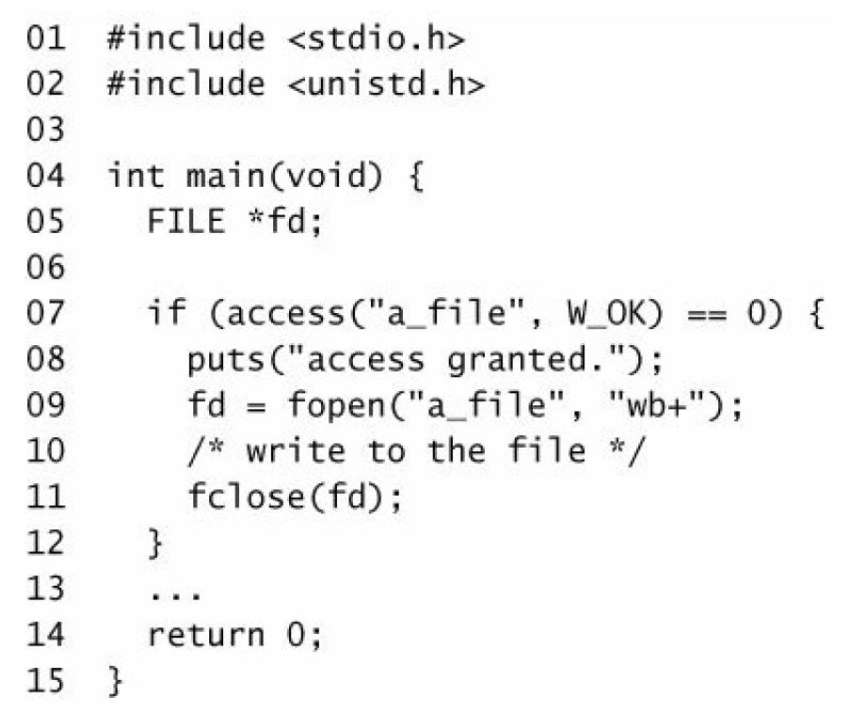
\includegraphics[width=0.5\textwidth, keepaspectratio]{capitoli/secure_coding/img/cap_6/esempio_file.png}
\end{wrapfigure}

Abbiamo un puntatore a file \verb|*fd|.
Controllo se il file è aperto in scrittura (se ho i diritti per scriverci).
Alla linea 7 avviene il check mentre alla 9 il time-to-use.
Tra questi due momenti c'è una race condition.
Supponiamo che il processo stia girando con i \textbf{diritti di root}.
Ricordiamo che una delle operazioni più importanti da compiere quando si configura
un sistema Unix è quello di disabilitare l'utente root.
Immaginiamo però di aver dimenticato questa parte. Andremo a vedere come sfruttare
questa vulnerabilità.
Supponiamo che nella race window entri qualcuno con i comandi seguenti e li esegua in continuazione:

\begin{lstlisting}
    rm a_file
    ln -s /etc/shadow a_file
\end{lstlisting}

Il programma controlla dunque i diritti di accesso al file.
Se l'esito è positivo, si prosegue con il resto del codice, andando ad effettuare
le operazioni di scrittura sul file.
A questo punto \verb|a_file| viene cancellato e viene creato un link al file delle password,
che però ha lo stesso nome del file appena rimosso. Il processo va ad aprire \verb|a_file|,
ma è stato sostituito con il link e compie le azioni successive su di esso.
Siamo quindi riusciti a scrivere nel file \verb|/etc/shadow| sfruttando il codice
vulnerabile di questo programma.

\paragraph{Possibile soluzione:}
effettuare check e using insieme !
Una possibile soluzione che utilizza la funzione
\verb|open()| è quella di ricorrere ai flag \verb|O_CREAT| e \verb|O_EXCL|.
Se usati insieme, questi flag indicano alla funzione \verb|open()| di fallire
se il file specificato da \verb|nome_file| esiste già.
Non c'è possibilità che venga messo un link ad un altro file da parte di un
utente malintenzionato, prima che esso venga mandato in esecuzione.

\begin{figure}
    \centering
    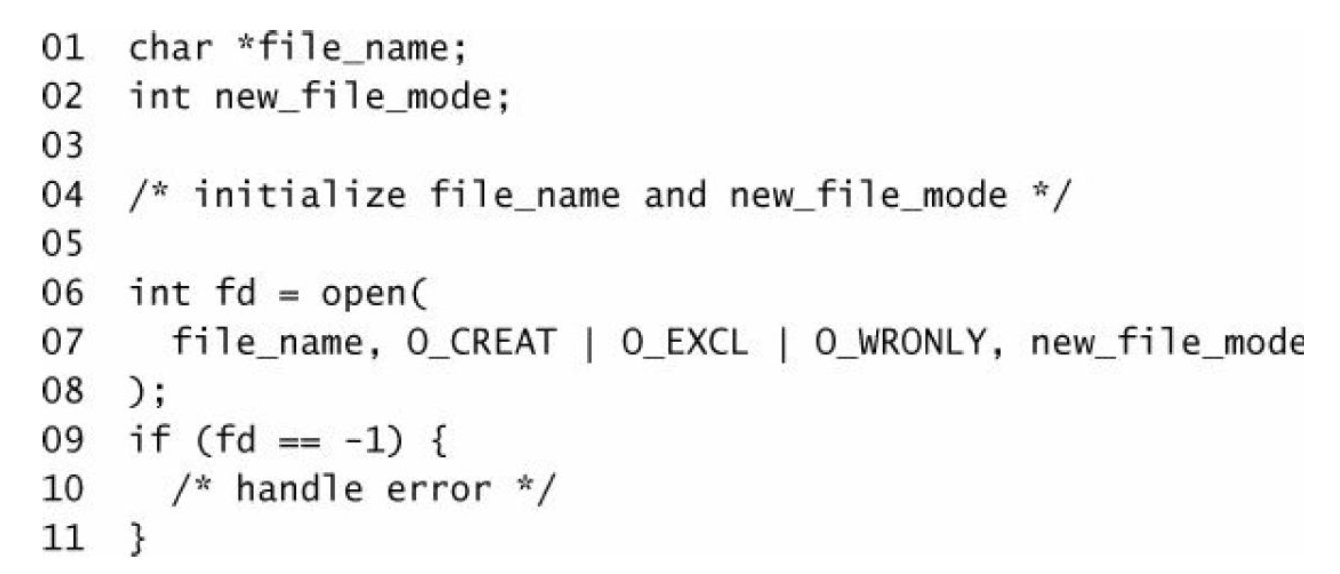
\includegraphics[width=10cm, keepaspectratio]{capitoli/secure_coding/img/cap_6/esempio_open.png}
    \caption{Possibile soluzione al problema TOCTOU.}
\end{figure}

\section{Prevenzione}

Per prevenire le race ai dati, quando due o più thread agiscono sullo stesso
oggetto devono utilizzare delle \textbf{primitive di sincronizzazione}.
C e C++ supportano diversi tipi di primitive di sincronizzazione, tra cui \textit{mutex},
\textit{condition variables} e \textit{lock variables}.
Ogni sezione critica appare atomica a tutti i thread opportunamente sincronizzati,
ad eccezione di quello che esegue la sezione critica.
Quando si lavora con i thread, non dobbiamo fare affidamento sul fatto che le istruzioni
vengano eseguite
esattamente nell'ordine in cui sono poste.
Le istruzioni assembly possono essere infatti riordinate dal

\begin{itemize}
    \item Processore durante l'esecuzione
    \item Compilatore durante l'ottimizzazione
\end{itemize}

Di seguito andremo a dare alcune definizioni per rendere più chiari i concetti appena elencati.

\paragraph{Definizione.}
Una \textbf{mutex} è una variabile che serve per la protezione delle sezioni critiche.
Le variabili condivise possono essere modificate da più thread.
Solo un thread alla volta può accedere ad una risorsa protetta da una mutex.
La mutex è un semaforo binario cioè può assumere 2 valori: 0 (occupato)
oppure 1 (libero).
Pensiamo alle mutex come a delle serrature:
il primo thread che ha accesso alla risorsa lascia fuori gli altri thread
fino a che non ha portato a termine il suo compito. La \textit{C standard library}
ci mette a disposizione le seguenti funzioni per lavorare con le mutex:

\begin{itemize}
    \item Funzioni per bloccare e rilasciare mutex:
          \begin{itemize}
              \item \verb|mtx_lock()|,
              \item \verb|mtx_unlock()|,
              \item \verb|mtx_trylock()|,
              \item \verb|mtx_timedlock()|.
          \end{itemize}
    \item Funzioni per la creazione di mutex:
          \begin{itemize}
              \item \verb|mtx_init()|
              \item \verb|mtx_destroy()|
          \end{itemize}
\end{itemize}

\paragraph{Definizione.}
I \textbf{lock guard} sono oggetti che fungono da wrap alle mutex per andare a
semplificarne l'utilizzo. Quando questo oggetto viene creato (generalmente in una
funzione), blocca automaticamente la mutex. Quando questo viene distrutto (generalmente
quando la funzione termina) rilascia automaticamente la mutex. Questo comportamento
cerca di risolvere dimenticanze del programmatore come non rilasciare la mutex quando
il thread ha terminato di lavorare con la risorsa condivisa.

\begin{figure}[H]
    \centering
    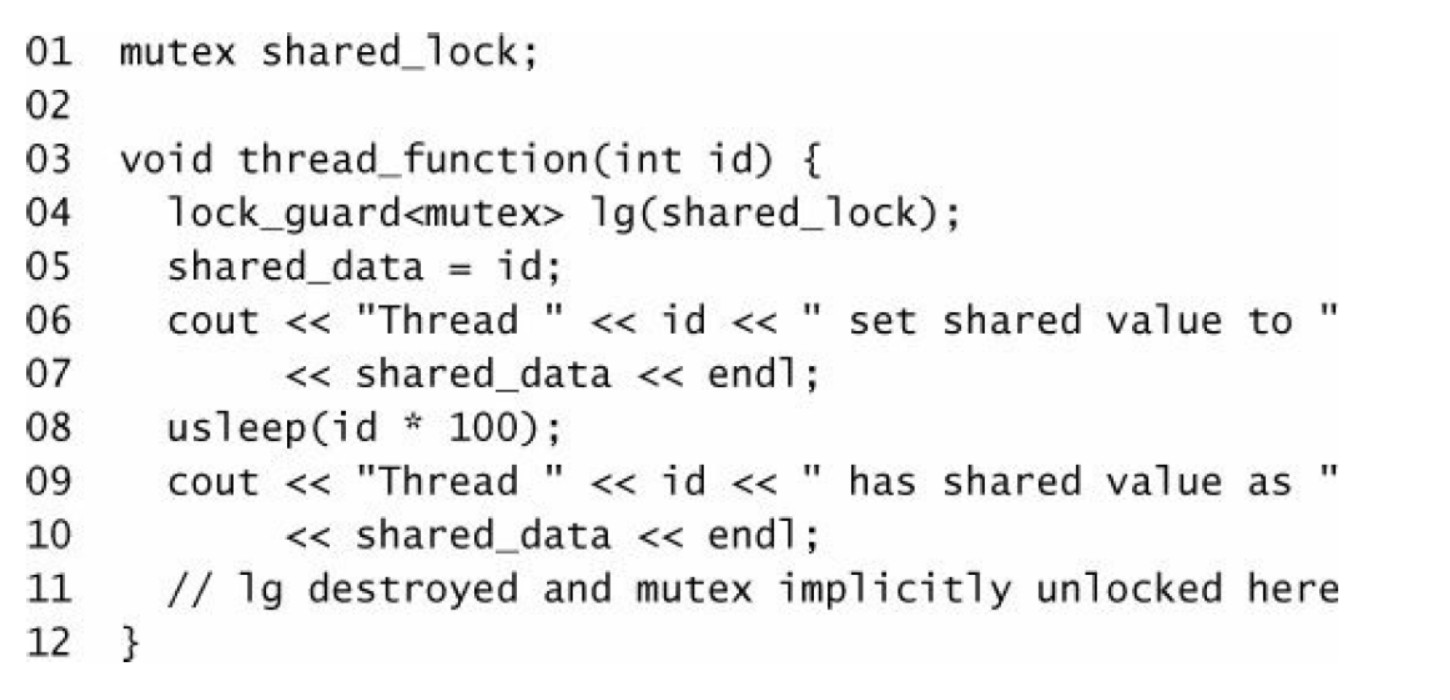
\includegraphics[width=10cm, keepaspectratio]{capitoli/secure_coding/img/cap_6/lockguard.png}
    \caption{Esempio di codice che sfrutta un lock guard.}
\end{figure}

\paragraph{Definizione.}
Un \textbf{atomic object} è un oggetto che garantisce che tutte le operazioni effettuate su di lui
siano \textit{atomiche}. Questa sua proprietà fa si che non può mai venire corrotto da azioni di
lettura e scrittura effettuate simultaneamente. In breve non possono esserci data race.

\begin{figure}[H]
    \centering
    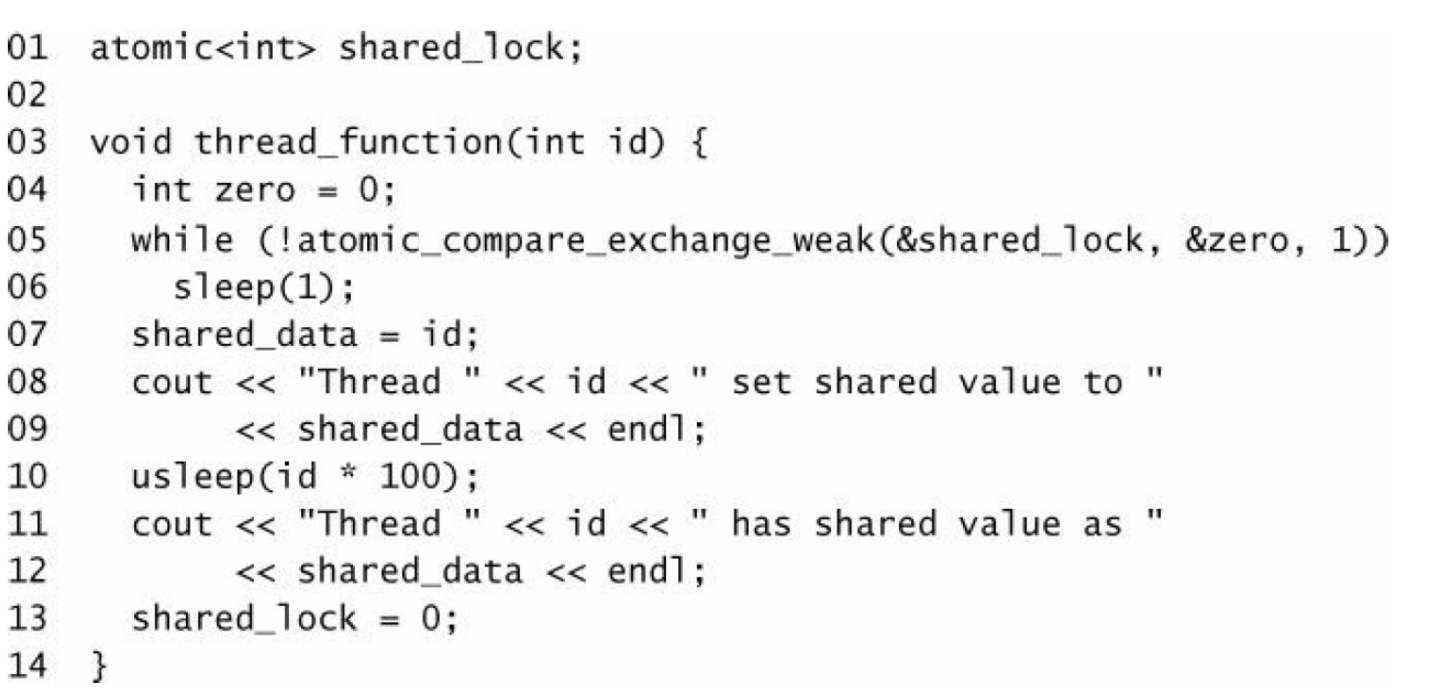
\includegraphics[width=10cm, keepaspectratio]{capitoli/secure_coding/img/cap_6/atomicobject.png}
    \caption{Esempio di codice che sfrutta un atomic object.}
\end{figure}

\paragraph{Definizione.}
Un \textbf{semaforo} è simile a una mutex, tranne per il fatto che
mantiene anche un contatore il cui valore viene dichiarato al momento dell'\\inizializzazione.
Di conseguenza, i semafori sono decrementati e incrementati piuttosto che bloccati e sbloccati.
Quando il contatore di un semaforo raggiunge lo 0, i tentativi successivi di decrementare
il semaforo si bloccano fino a quando il contatore non viene nuovamente incrementato.
Questo sta a segnalare che il massimo numero di thread che possono utilizzare la risorsa è
stato raggiunto.\ \\


Di seguito andremo ad elencare i principali problemi che possono verificarsi quando si lavora
in un ambiente con più thread che concorrono tra di loro.

\begin{itemize}
    \item Dimenticarsi di utilizzare il il lock quando si accede ai dati condivisi
          (non bloccare la risorsa quando vi si accede);
    \item Rilasciare prematuramente un lock. Non si è chiusa la race window, quindi
          possono ancora accadere race conditions;
    \item Generazione di Deadlock causati da:
          \begin{itemize}
              \item Uso improprio o selezione impropria di meccanismi di locking;
              \item Non sbloccare un lock o cercare di riacquistarne uno già mantenuto;
              \item In poche parole ci si dimentica di rilasciare la mutua esclusione;
          \end{itemize}
    \item Mancanza di \textit{fairness} (equità) tra i processi.
          Alcuni entrano più volte nella mutua esclusione, altri meno;
    \item Starvation;
    \item Livelock (stare continuamente in attesa senza procedere);
    \item Non assumere mai che i thread vengano eseguiti in un particolare ordine.
\end{itemize}

\subsection{Memory Fencing}

“Fencing” vuol dire \textbf{barriera}, cancello.
In questo esempio la scrittura e la lettura vengono riorganizzate dal compilatore.
È possibile che sia \verb|r1| che \verb|r2| siano settati a 0.
Infatti, nel thread 2 (se nel primo \verb|x| non è ancora stata scritta) \verb|r2|
diventerà uguale a 0.

\begin{figure}[H]
    \centering
    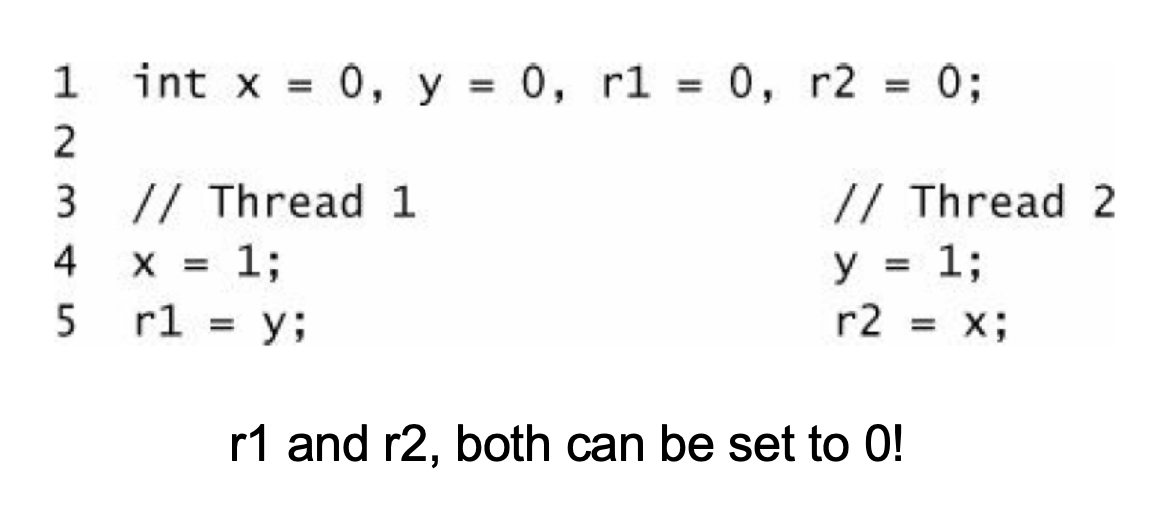
\includegraphics[width=10cm, keepaspectratio]{capitoli/secure_coding/img/cap_6/nofance.png}
    \caption{Esempio di codice per cui sia r1 che r2 possono essere 0.}
\end{figure}

Una possibile soluzione è rappresentata dal \textit{memory fencing}:

\begin{figure}[H]
    \centering
    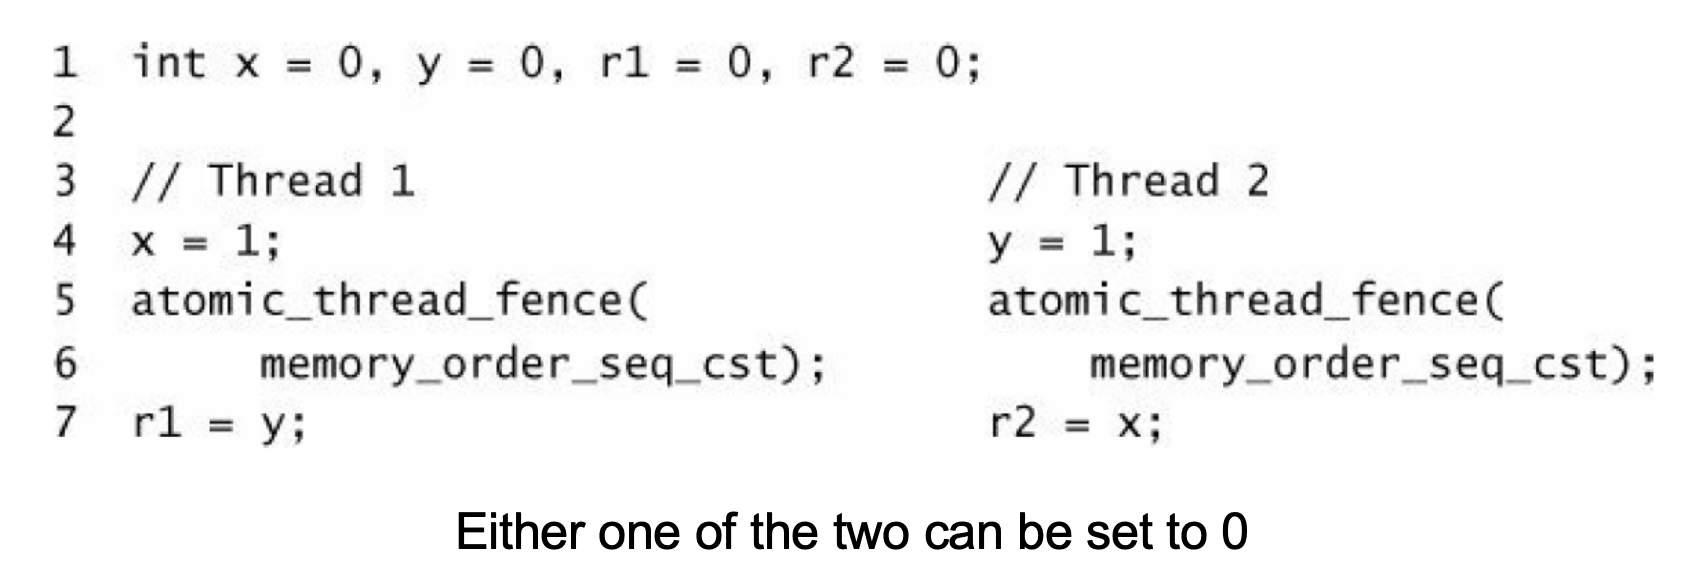
\includegraphics[width=10cm, keepaspectratio]{capitoli/secure_coding/img/cap_6/sifance.png}
    \caption{Possibile soluzione con memory fencing.}
\end{figure}

Esiste una speciale funzione \verb|atomic_thread_fence| (alla linea 5) che
forza ad apportare le modifiche in memoria.
Per cui saremo certi del fatto che i cambiamenti verranno apportati.
A questo punto solo uno tra \verb|r1| e \verb|r2| sarà uguale a 0,
dipende chi viene eseguito per primo.


\subsection{File Locks}

È possibile utilizzare la creazione di un file come lock.
Tutti i processi controllano se il file è già stato creato.
Se così è, vanno in “sleep”. I vari controlli avvengono chiaramente in mutua esclusione.
Alla fine, il primo processo che termina cancella il file;
il primo che invece si sveglia e si rende conto del fatto che non c'è più, lo ricrea.
In realtà questa soluzione non è consigliata: è meglio usare strutture apposite, tipo mutex e simili.

\subsection{Tools}

Esistono dei tools per controllare se vi sono race condition.
Uno strumento di \textbf{analisi statica} analizza il software per ritrovarle,
senza eseguirlo effettivamente.
In generale la condition detection è un problema è NP completo (esponenziale).
Diventa sempre più complesso con l'aumentare dei flussi di controllo.
Per questo motivo gli strumenti di rilevamento statico delle race condition forniscono
un'identificazione approssimativa.
Di conseguenza, tutti gli algoritmi di analisi statica sono soggetti ad alcuni falsi
negativi e falsi positivi.
Esiste il \textit{Clang thread Safety Analysis} (Google) che esegue un controllo
per capire se sono presenti race conditions:

\begin{lstlisting}
    clang -c -Wthread-safety example.cpp
\end{lstlisting}

Gli strumenti di rilevamento \textbf{dinamico} delle race condition riescono a superare alcuni
problemi degli strumenti statici, eseguendo effettivamente il programma.
Ci sono meno falsi positivi. Tuttavia, gli svantaggi del rilevamento dinamico sono:

\begin{itemize}
    \item Il fatto che non tiene conto dei percorsi di esecuzione non eseguiti;
    \item spesso c'è un overhead di tempo di esecuzione.
\end{itemize}

Possibili tools sono: Intel Inspector (a pagamento) e Helgrind
(parte di Valgrind, cioè una suite di 6 tools differenti).
